%%%%%%%%%%%%%%%%%%%%%%%%%%%%%%%%%%%%%%%%%%%%%%%%%%%%%%%%%%%%%%%%%%%%%
%
% CSCI 1430 Writeup Template
%
% This is a LaTeX document. LaTeX is a markup language for producing
% documents. Your task is to fill out this
% document, then to compile this into a PDF document.
%
% TO COMPILE:
% > pdflatex thisfile.tex
%
% For references to appear correctly instead of as '??', you must run
% pdflatex twice.
%
% If you do not have LaTeX and need a LaTeX distribution:
% - Departmental machines have one installed.
% - Personal laptops (all common OS): www.latex-project.org/get/
%
% If you need help with LaTeX, please come to office hours.
% Or, there is plenty of help online:
% https://en.wikibooks.org/wiki/LaTeX
%
% Good luck!
% James and the 1430 staff
%
%%%%%%%%%%%%%%%%%%%%%%%%%%%%%%%%%%%%%%%%%%%%%%%%%%%%%%%%%%%%%%%%%%%%%
%
% How to include two graphics on the same line:
%
% \includegraphics[\width=0.49\linewidth]{yourgraphic1.png}
% \includegraphics[\width=0.49\linewidth]{yourgraphic2.png}
%
% How to include equations:
%
% \begin{equation}
% y = mx+c
% \end{equation}
%
%%%%%%%%%%%%%%%%%%%%%%%%%%%%%%%%%%%%%%%%%%%%%%%%%%%%%%%%%%%%%%%%%%%%%%%%%%%%%%%%%%%%%%%%%%%%%%%%

\documentclass[11pt]{article}

\usepackage[english]{babel}
\usepackage[utf8]{inputenc}
\usepackage[colorlinks = true,
            linkcolor = blue,
            urlcolor  = blue]{hyperref}
\usepackage[a4paper,margin=1.5in]{geometry}
\usepackage{stackengine,graphicx}
\usepackage{fancyhdr}
\setlength{\headheight}{15pt}
\usepackage{microtype}
\usepackage{times}
\usepackage{booktabs}

% python code format: https://github.com/olivierverdier/python-latex-highlighting
\usepackage{pythonhighlight}

\frenchspacing
\setlength{\parindent}{0cm} % Default is 15pt.
\setlength{\parskip}{0.3cm plus1mm minus1mm}

\pagestyle{fancy}
\fancyhf{}
\lhead{Project 3 Writeup}
\rhead{CSCI 1430}
\rfoot{\thepage}

\date{}

\title{\vspace{-1cm}Project 3 Writeup}


\begin{document}
\maketitle
\vspace{-2cm}
\thispagestyle{fancy}

% \section*{Instructions}
% \begin{itemize}
%     \item Provide an overview about how your project functions.
%     \item Describe any interesting decisions you made to write your algorithm.
%     \item Show and discuss the results of your algorithm.
%     \item Feel free to include code snippets, images, and equations.
%     \item List any extra credit implementation and result (optional).
%     \item Use as many pages as you need, but err on the short side.
%     \item \textbf{Please make this document anonymous.}
% \end{itemize}

\section*{Project Overview}

In this project, scene recognition was performed using three different methods, starting with very simple methods -- tiny images and nearest neighbor classification -- and then move on to more sophisticated methods -- bags of words and linear classifiers learned by support vector machines. The accuracy for the BoW/SVM can reach 76.7\%, while for BoW/NN, Tiny/SVM, Tiny/NN are 63.1\%, 25\%, 22.2\%, respectively.

\section*{Implementation Detail}

The implementation order is following the implementation strategy part on \hyperlink{https://browncsci1430.github.io/webpage/proj3_scenerecognition/}{project website}. The accuracy results will be discussed in the Result section. Any implementations for extra credits will be discussed in the Extra Credit section.

All image operations have been optimized for parallel using multiple CPUs with the help of \verb|Parallel()| from \verb|joblib| package, which reduces the execution time dramatically to 22s on Gradescope, compared to the means of other students' execution time, 200s or so.

\subsection*{Explaination for implementation of get\_tiny\_images()}
First, images are collected using \verb|imread()| using one for loop. Then, the resize operation are done in \verb|Parallel()| by calling the \verb|tiny_feature()| which will resize the image to 16$\times$16 shape.

\subsection*{Explaination for implementation of build\_vocabulary()}
Similar to \verb|get_tiny_images|, images are collected in one for loop in the begining. Then I have implemented four descriptors to construct the feature space for the images, hog, gaussian\_pyramid, gist and daisy. The last three will be discussed in the Extra Credit section.

The detail for hog descriptors is in \verb|hog_feature()| function, \verb|hog()| function from \verb|sklearn| package is used and the parameters have been optimized for the best performance, e.g. \verb|pixels_per_cell_dim| is 8 and \verb|cells_per_block_dim| is 2. Then the features returned from \verb|hog()| are reshaped to (-1, \verb|cells_per_block_dim| $\times$ \verb|cells_per_block_dim| $\times$ 9)

Then the features obtained for all images are clustered using \verb|MiniBatchKmeans()| with the number of clusters set as 200, i.e. the size of our vocabulary is 200.

\subsection*{Explaination for implementation of get\_bags\_of\_words()}
Similar to \verb|build_vocabulary|, images are collected in the begining. To utilized the \verb|Parallel| function, I implement \verb|generate_feats| to encode every image with the vocabulary we generated in the previous function.

To make it consistent with the construction of vocabulary, descriptors type here are the same as those used in \verb|build_vocabulary|. Once the features for each image are obtained. The euclidean distances are calculated using \verb|cdist|. The each feature is labeled by the nearest word. Then we simply count the histogram of the feature labels and return it as the final feature of the image. "soft assignment" is also implemented and will be discussed in Extra Credit section.

\subsection*{Explaination for implementation of svm\_classify()}

Multiple SVM methods have been tested here, such as poly, sigmoid, rbf and che-sqr. The results will be discussed in Extra Credit section.

\subsection*{Explaination for implementation of nearest\_neighbor\_classify()}

In this function, the feature of the image is labeled by the nearest point. For k points, the label of the image will be the label that appears most times among these nearest k points. Different k values have been tested and weighted votes have been implemented to improve the performance of kNN method. The detail will be discussed in Extra Credit section.

\section*{Result}

Here we presented the result with optimized parameters. The code here is the same as what we submit to Gradescope, i.e. the SVM method, the hog parameters etc. For \verb|bag_of_words|, we use hog and gaussian\_pyramid together to construct vocabulary and encode images. In \verb|get_bags_of_words|, we use soft assignment to obtain the feature of the image. We use poly SVM for \verb|svm_classify| and $k=15$ with weighted votes for \verb|nearest_neighbor_classify|

\begin{table}[h]
    \centering
    \begin{tabular}{lr}
        \toprule
        Models             & Accuracy(\%) \\
        \midrule
        bag\_of\_words/SVM & 78.267       \\
        bag\_of\_words/NN  & 63.333       \\
        tiny\_image/SVM    & 24.333       \\
        tiny\_image/NN     & 22.467       \\
        \bottomrule
    \end{tabular}
    \caption{Performance of different methods in provided dataset}
    \label{acc}
\end{table}

\begin{figure}[htbp]
    \centering
    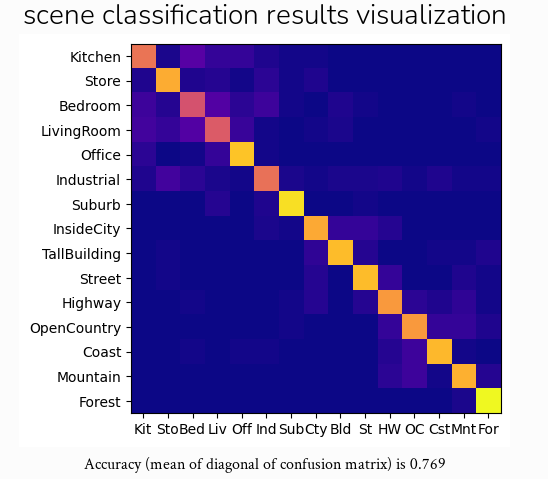
\includegraphics[scale=0.7]{confusion.png}
\end{figure}

\begin{figure}[htbp]
    \centering
    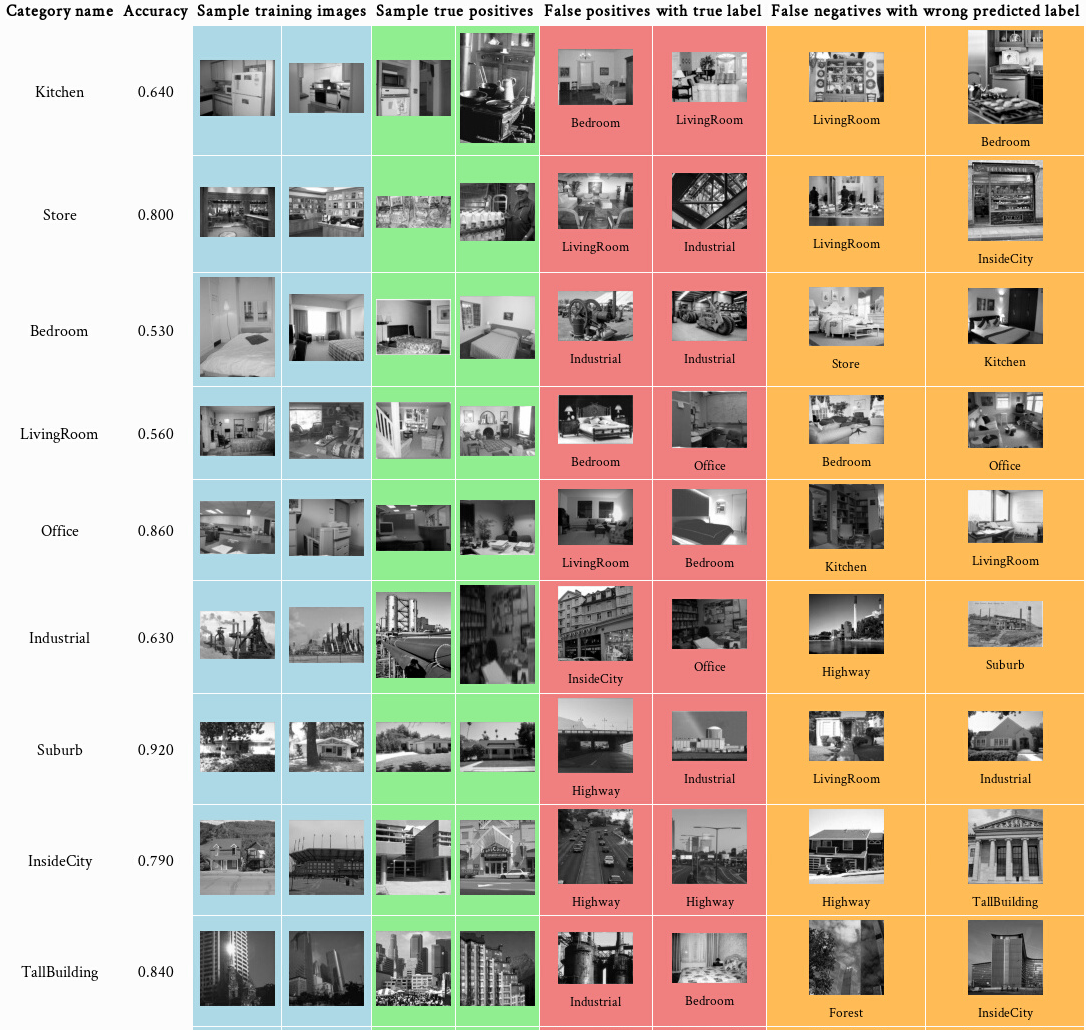
\includegraphics[scale=0.6]{scence_table.png}
    \caption{For more scences details, please check the index.html file}
    \caption{For more scences details, please check the index.html file}
\end{figure}

\section*{Extra Credit (Optional)}
\begin{enumerate}
    \item Feature representation extra credit
          \begin{itemize}
              \item \textbf{Sampling features from different levels of a Gaussian pyramid}: the implementation detail can be found in \verb|gaussian\_pyramid\_feature()|. 
              
              Simply speaking, \verb|pyramid_gaussian| funtion in \verb|sklearn| is used to constructed the image pyramid. Then images are resized back the original image size and features are constructed based upon these image patches. This method does improve the accuracy by about 4\%. Therefore, I used it combined with hog as my final submission.
              \item \textbf{Add gist descriptors and consider with other existing descriptors together for vocabulary}: 
              
              the implementation detail can be found in \verb|gist_feature()|. Intuitively, GIST summarizes the gradient information (scales and orientations) for different parts of an image, which provides a rough description (the gist) of the scene.Given an input image, the gist descriptor is computed by
                    \begin{enumerate}
                        \item Convolve the image with 32 Gabor filters at 4 scales, 8 orientations, producing 32 feature maps of the same size of the input image.
                        \item Divide each feature map into 16 regions (by a 4x4 grid), and then average the feature values within each region.
                        \item Concatenate the 16 averaged values of all 32 feature maps, resulting in a 16x32=512 GIST descriptor.
                    \end{enumerate}
                    As the resulting feature for the image is (512,), to combine with hog features, I reshape the gist feature to (-1, 36) after throwing away the final 8 dimension in original vector as $512 \% 36=8$. Here is the result for combining hog, gaussian-pyramid and gist descriptors. The parameters are the same as provided in Result section.
                    \begin{table}[h]
                        \centering
                        \begin{tabular}{lr}
                            \toprule
                            Models             & Accuracy(\%) \\
                            \midrule
                            bag\_of\_words/SVM & 78.267       \\
                            bag\_of\_words/NN  & 63.333       \\
                            tiny\_image/SVM    & 24.333       \\
                            tiny\_image/NN     & 22.467       \\
                            \bottomrule
                        \end{tabular}
                        \caption{Performance of different methods using gist in provided dataset}
                        \label{multi_descriptor}
                    \end{table}
          \end{itemize}
    \item Feature quantization and bag of words extra credit
          \begin{itemize}
              \item \textbf{Use "soft assignment" to assign visual words to histogram bins}: below the corresponding code for soft assignment part. The distances between image features and vocabulary are filtered with gaussian formula. Each visual word will cast a distance-weighted vote to multiple bins. Thus, the further distance between the feature and the word, the less contribution the word to the final bincount number. This will improve the accuracy by about 3\%.
                    \begin{python}
sigma = 0.05
distances = np.exp(-(distances ** 2) / (sigma ** 2))
distances = distances / np.sum(distances, axis=1)[:, np.newaxis]
feats = np.sum(distances, axis=0)
                    \end{python}
          \end{itemize}
    \item Classifier extra credit
          \begin{itemize}
              \item \textbf{Train the SVM with different kernels}:
              
              the implementation detail can be found in \verb|svm_classify()|.
              Different SVM models have been tested here using \verb|SVC| with different kernels. The performance comparison is presented below.
                    \begin{table}[h]
                        \centering
                        \begin{tabular}{lr}
                            \toprule
                            Models     & Accuracy(\%) \\
                            \midrule
                            Linear     & 75.800       \\
                            poly       & 78.267       \\
                            sigmoid    & 59.933       \\
                            rbf        & 72.733       \\
                            anova/chi2 & 57.867       \\
                            \bottomrule
                        \end{tabular}
                        \caption{Performance of different methods using different SVM method on the same vocabulary}
                        \label{svm}
                    \end{table}
          \end{itemize}
    \item \textbf{Spatial Pyramid representation and classifier}: 
    
    the implementation detail can be found in \verb|build_spatial_pyramid()| and \verb|spatial_pyramid_matching()|.

    This feature is not fully implemented as I haven't successfully configured how to trace back the location of feature generated by hog. In the \hyperlink{https://inc.ucsd.edu/~marni/Igert/Lazebnik_06.pdf}{paper}, the dense SIFT descriptor is used and thus the location of each feature in the image is the center point location. However, for hog descriptor, the block will overlap with each other and the returned feature vectors are flatten and reshaped, which makes it difficult to figure out how to assign the location of each feature back to the image. Thus, in my implementation, I assume that there exists one function \verb|locate_descriptors()| that can locate the corresponding feature vector in the image and return the positions.
    
    The principle of spatial pyramid representation is that counting the feature label in different scales, and adding these count together with weigting levels' count to a final feature for the image (See \verb|spatial_pyramid_matching()| for weights assignment). Once we could locate the positions of the features and counting them by dividing the original image to different sections. The final feature can be obtained by summing them up.

    \item Experimental design extra credit
          \begin{itemize}
              \item \textbf{experiment with many different vocabulary sizes}: the performance of model with different vocabulary size is presented below. However, the performance is not stable as the results will fluctuate about 2\% due to the randomalization of Kmeans and SVM. We could see that increase the vocabulary size could increase accuracy at first. However, larger vocabulary size doesn't guarantee better performance.
                    \begin{table}[h]
                        \centering
                        \begin{tabular}{lrrrrrrrr}
                            \toprule
                            Vocab Size         & 10 & 20     & 50     & 100    & 200    & 400    & 1000   & 10000 \\
                            \midrule
                            bag\_of\_words/SVM & 54 & 63.533 & 71.933 & 74.267 & 76.867 & 74.933 & 81.267 & 77.0  \\
                            bag\_of\_words/NN  & 49 & 54.4   & 59.467 & 61.267 & 63.133 & 60.4   & 65.133 & 53.6  \\
                            \bottomrule
                        \end{tabular}
                        \caption{Performance with different vocabulary size}
                        \label{svm}
                    \end{table}

              \item \textbf{report performance on the 397-category \hyperlink{https://vision.princeton.edu/projects/2010/SUN/}{SUN database}}.

          \end{itemize}
\end{enumerate}

\end{document}
